\section{Bessel functions}
\label{sec:bessel}

\textbf{Illustrates}: Special functions library, array manipulations
to check recursion relation.


In this exercise, you will verify a few simple relations involving the Bessel
functions of the first kind.  The important relations to keep in mind are the
asymptotic form of $J_n(x)$ for $x>>n$:

\begin{equation}
J_n(x) \approx \sqrt(\frac{2}{\pi x})\cos(x-(n\frac{\pi}{2}+\frac{\pi}{4}))
\end{equation}

%
and the recursion relation

\begin{equation}
J_{n+1}(x) = \frac{2n}{x} J_n(x)-J_{n-1}(x)
\end{equation}

\begin{figure}
\begin{centering}
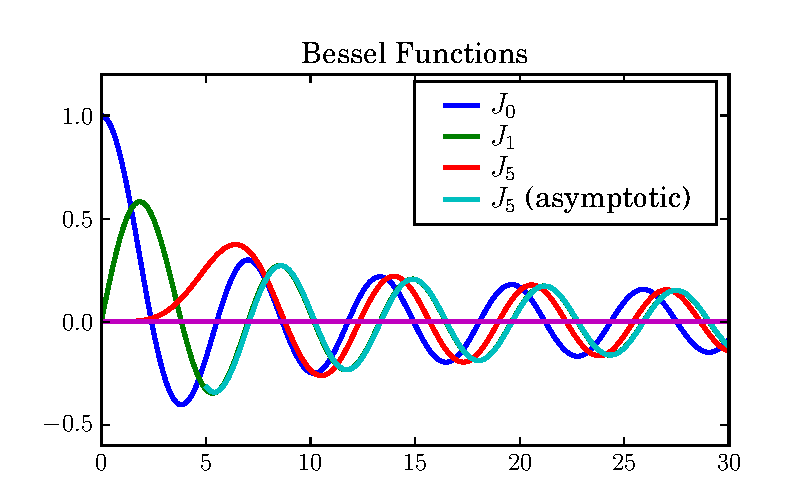
\includegraphics[width=5in]{fig/bessel_functions}
\par
\end{centering}


\caption{\label{fig:bessel_functions}A few Bessel functions.}

\end{figure}



\begin{figure}
\begin{centering}
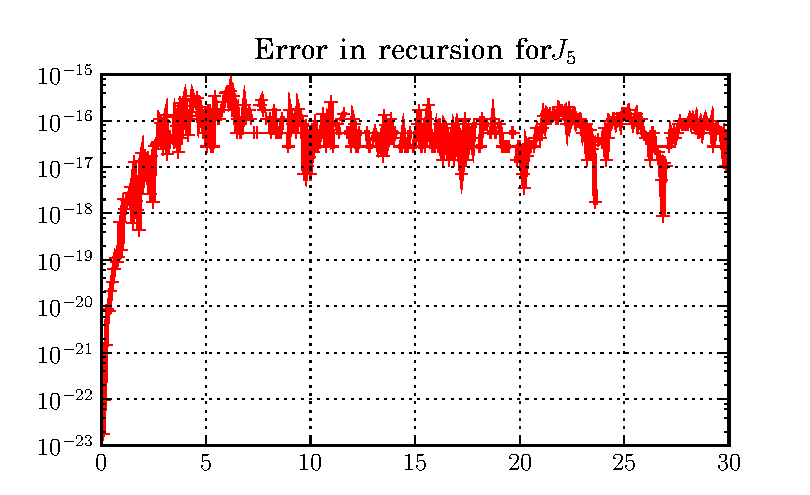
\includegraphics[width=5in]{fig/bessel_error}
\par
\end{centering}


\caption{\label{fig:bessel_error}Numerical error for $J_5$.}

\end{figure}

Once you get the code to run, you should see two figures like
Figure~\ref{fig:bessel_functions} and Figure~\ref{fig:bessel_error}.

\lstinputlisting[label={code:bessel},caption={IGNORED}]{problems/bessel.py}
